% This is the master file of the folder structure. In order to compile your document, run this file. In most LaTeX editors, the master file can be specified such that the document can also be compiled from the other .tex files (in the docs folder).

% First, the preamble needs to be called. This contains all the 'under the hood' stuff for your document.
% This file contains your LaTeX preamble. A preamble is a part of your document where all required packages and macros can be defined. This needs to be done before the \begin{document} command.

% Documentclass:
% Standard LaTeX classes are: article, book, report, slides, and letter. These cover the basis, but are not best. More advanced users might want to try out the KOMA classes or the memoir class. Optional arguments: 10pt. The font size of the main content is set to 10pt with the option between [].
\documentclass[10pt]{article}

% Geometry:
% The papersize of the document is defined with the geometry package. Here, the size is set to A4 with a4paper. Other possibilities are a5paper, b5paper, letterpaper, legalpaper and executivepaper.
\usepackage[a4paper]{geometry}
\usepackage{multicol}
\usepackage[super]{natbib} 

% AMS math packages:
% Required for proper math display.
\usepackage{amsmath,amsfonts,amsthm}

% Graphicx:
% If you want to include graphics in your document, the graphicx package is required.
\usepackage{graphicx}

% Booktabs:
% The booktabs package is needed for better looking tables. 
\usepackage{booktabs}

% SIunitx:
% The SIunitx package enables the \SI{}{} command. It provides an easy way of working with (SI) units.
\usepackage{siunitx}

% URL:
% Clickable URL's can be made with this package: \url{}.
\usepackage{url}

% Caption:
% For better looking captions. See caption documentation on how to change the format of the captions.
\usepackage{caption}

% Hyperref:
% This package makes all references within your document clickable. By default, these references will become boxed and colored. This is turned back to normal with the \hypersetup command below.
\usepackage{hyperref}
	\hypersetup{colorlinks=false,pdfborder=0 0 0}

% Cleveref:
% This package automatically detects the type of reference (equation, table, etc.) when the \cref{} command is used. It then adds a word in front of the reference, i.e. Fig. in front of a reference to a figure. With the \crefname{}{}{} command, these words may be changed.
\usepackage{cleveref}
	\crefname{equation}{equation}{equations}
	\crefname{figure}{figure}{figures}	
	\crefname{table}{table}{tables}

% The title page is created with the command \maketitle which needs to be placed after the \begin{document} command. To create the titlepage, some entries are needed: the name of the autor is defined by \author{}, the title by the entry \title{} and the date by the command \date{}. Note that the current date is displayed with \today.
\author{ 
Manuel F. Graf\\
  \texttt{grafm@cip.ifi.lmu.de}
  \and
  Michael A. Prummer\\
  \texttt{prummer@cip.ifi.lmu.de}
}
\title{Design of a Multiplayer Exergame for a Biofeedback System using Unity 3D
}
\date{\today}


\begin{document}

%\tableofcontents

\maketitle

\textbf{\section{abstract}
The Biofeedback System developed at the German Heart Center focuses on the creation of different games that may help to motivate children in the rehabilitation process after surgery, monitoring their vital parameters and adapting to specific conditions.

This paper describes the design and integration of a multi-player video racing ‘exergame’,  controlled via an ergometer and motion sensor, that utilizes the display of Biofeedback to increase or decrease the players physical activity depending on their current heart rate. A preliminary study with young healthy students showed that an aerobic exercise level can be reached, even during short sessions.
\cref{Goe210}
}

\begin{multicols}{2}

\section{Introduction}
Biofeedback is a relatively new method of treatment for mainly psychosomatic diseases. It can be used in many different ways through visualizing information about the physiological functions of the body. Biofeedback can be applied using various types of data, such as heart rate, brainwaves, body temperature or skin conductance of a patient. This data may help to improve the health and performance of an individual during a physical exercise or a treatment. Visualizing the participants vital parameters improves the perception of his own body and thus his health. 
By adapting to the given feedback patients can learn to affect their own body functions.\cite{BF2007} The recorded biofeedback data of patient during an exercise could be visualized and analyzed across multiple sessions. 

Besides this, Biofeedback could also be used to promote and motivate exercise for rehabilitation. Therefore, the biofeedback system can be combined with interactive applications, which hide the exhausting task of exercising behind a video game. Most things could be done more easily if we think of it as a game instead of work. Especially for rehabilitation, it may help to make boring exercises more entertaining, that have to be repeated continuously over a very long period, but are crucial for physical recovery. In order to combine interactive games with
exercise and biofeedback, we will introduce the concept of exergames (EG) and serious games (SG).
\begin{figure}[H]
  \centering
    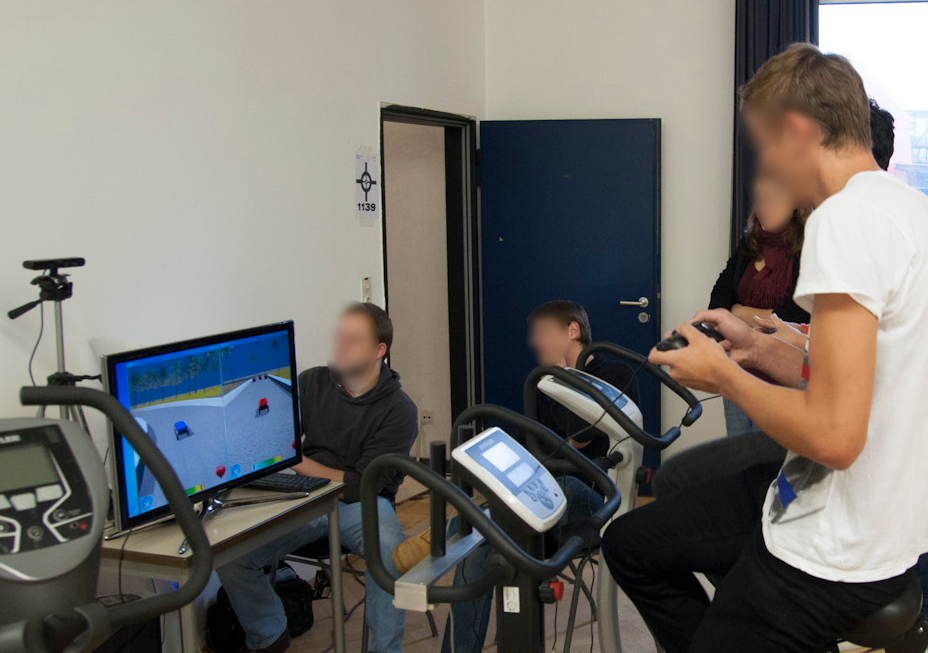
\includegraphics[width=0.5\textwidth]{BATesting_setup}
 \caption{Testing of the first prototype}
\end{figure}
Games designed for a specific purpose, teaching a skill or educate can be referred as serious games. \cite{Derryberry} Serious games are a steady growing and relevant market since video games get more accepted in society. \cite{SGIndustry} The game prototype we seek to develop for the biofeedback system at the “Deutsches Herzzentrum” (DHZ), can be classified as a serious game based on the player movement or more specific, an exergame. “The activity of playing video games that involve physical exertion can be seen as a form of exercise.” \cite{ExergameDef}

\section{Related Work}
There are many successful commercial “exergame platforms” like the Nintendo Wii or Wii Fit. Studies about the efficiency of the Wii according to the exercise, mostly shows different results. \cite{Baranowski2012} The major problem with most of the consumer systems is that the patient could easily adopt a strategy to trick the system to be successful in the game. Accordingly, we have to use our own motion tracking system with a camera to avoid such behavior in first place. Thus, exergames are not full replacements for real sports, they can be a great support in improving balance, endurance or help be more aware of specific problems. There are also many scientific evaluated studies from Baranowski \cite{Baranowski2008} and Kretschmann \cite{Kretschmann2010}, which have shown positive health related behavior changes in working together with video game setups.

Information we gathered from the evaluation of the previously developed exergames at the DHZ showed that single-player video games lacked the needed methods to sustain motivation. Playing the games for the first time could be a lot of fun while the concept of controlling the game over the biofeedback sensors is new to the player. But as already stated, this setup won't work quite well in keeping up the long term motivation for proceeding sessions.


\section{Motivational Aspects}

A big challenge in creating a high qualitative exergame is to make it replayable and keep up a steady motivation over a longer period of time while still maintaining a steady physical energy expenditure. 
Stuart Gray researched the connection between physical extent in exergamess and the motivational pull of head-to-head and leader board competitive games \cite{Gray2013} by analyzing the results of different studies which vary in their results regarding the effect of multiplayer competitive games on players motivation. His conclusion was that competitive gameplay can have either a negative or positive effect on energy expenditure depending on how competitive participants are. Still, his main study showed that participants who played any competitive game mode spent significantly more time in anaerobic training zones, suggesting that competitive conditions are more effective for energy expenditure than non-competitive conditions. Thus our goal was to develop a multiplayer racing exergame, which could be played together with up to eight players or an artificial intelligence.

We also tried to improve the game experience through controlling the karts by intuitive controls via motion sensor to increase perceived competence and thus intrinsic motivation \cite{Ryan2006SDT}.
\begin{figure}[H]
  \centering
    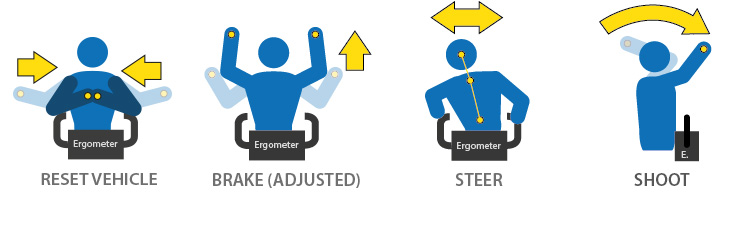
\includegraphics[width=0.4\textwidth]{gestures3}
 \caption{Motion sensor interaction}
\end{figure}
Observation of a Preliminary study with 18 students of the \emph{University of Applied Sciences Munich} to test the interaction concept has shown that the motion sensor controls were accepted and had positive effects on the fun factor and replay motivation of the game. Because of sensor failures and difficulties with input delays which led to overcompensation in countersteering and early abortion of the sessions the collected training data was inconclusive. Despite that and the fact that cycling while steering the vehicle by upper body inclination was very hard task to accomplish, most participants stated they wanted to replay the game.

The Implementation of various game elements, such as weapons system or collectable items, similar to the classic, well known combat racing game \emph{ Super Mario Kart} \cite{NitendoWiiMario} should further enhance game experience and lower initial learning effort. 

To balance the gameplay and even put the chances to win between skilled and non skilled video gamers, the current racing position affects what kind of powerups the player can obtain. While the leading player receives only the weakest power-ups, the player at the last rank will more likely receive strong power-ups which have a huge impact on the current game state, allowing them to catch up fast.

\begin{figure}[H]
  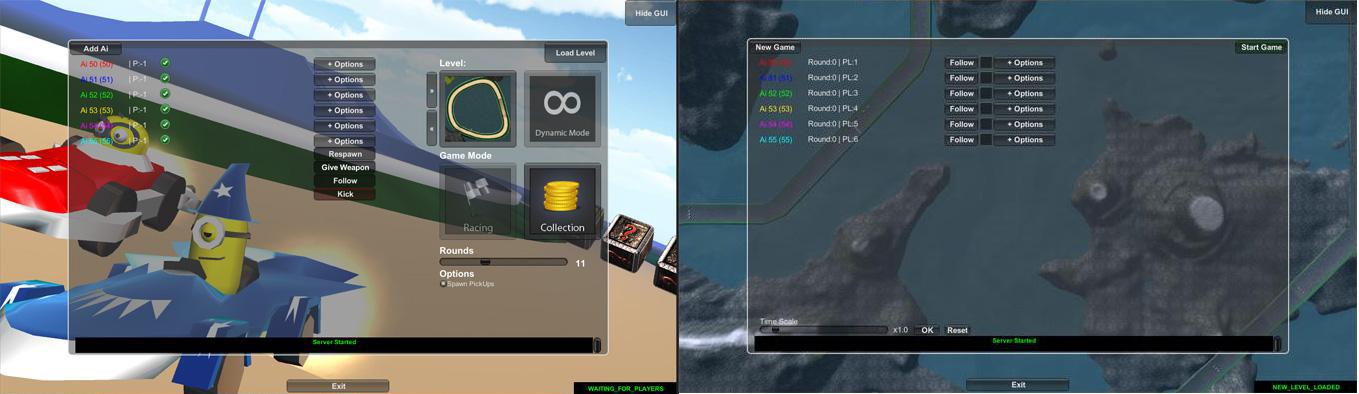
\includegraphics[width=0.5\textwidth]{ingame}
  \caption{Server game controls}
\end{figure}


The game prototype had to be developed with the Unity3D game engine, based on the experience and tools of former developed games at the DHZ. The game should provide an initial motivation to start with exercising and support a better long term motivation through the multiplayer extension. Therefore, we wanted the game to be appropriate for the longer task of rehabilitation, especially with the target group of children and adolescents. 

\section{Input Devices and Sensors}
The biofeedback system game setup consists of two common ergometers, a motion sensor and a belt for measuring heart rate and respiration. 
Other considerable parameters, which could affect the game are the cycling speed of the ergometers, respiration values and motion tracking. The ergometer standard RPM output values are normally measured by the momentum of the internal flywheel, so it will still produce data even if the patient stopped cycling. Since our application needed the actual cycling, we modified the measurement of rounds per minute (RPM) of the ergometers by tracking the cycle speed with magnets clamped behind the paddle. The game is played cycling on an ergometer and could either be controlled over the motion sensor or the game pad.

\begin{center}
\newcolumntype{C}[1]{>{\raggedright\let\newline\\\arraybackslash\hspace{0pt}}m{#1}}

\begin{tabular}{ | C{2cm}  | C{4.25cm} | } \hline
	% Heading    
    Sensor & Output Parameter \\ \hline
	% Row 1
 	Kettler Ergometer & Cycling speed in RPM (Integer) \\ \hline
	% Row 2 	
    CSL Gamepad & Button states (Integer) Analog-Stick Values (Float) \\ \hline
   	% Row 3
    Zephyr Bioharness Strap & Heart-Rate and Respiration (Integer) \\ \hline
	% Row 4
    Asus Xtion Motion Sensor & Tracking of the upper body movements (Integer) \\ \hline    
    \end{tabular}

\end{center}

\begin{figure}[H]
  \centering
    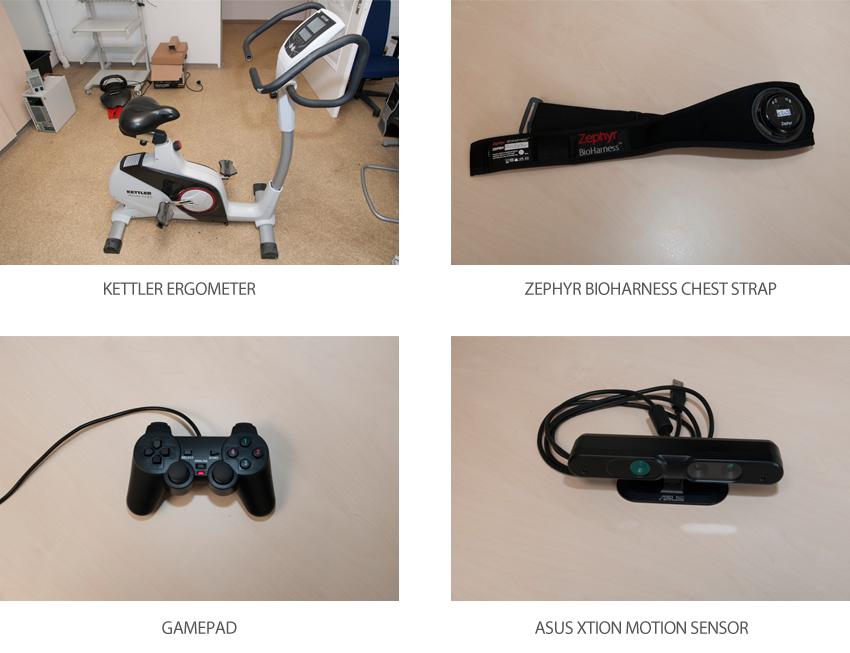
\includegraphics[width=0.4\textwidth]{sensors}
 \caption{Sensors used}
\end{figure}

To connect all required medical sensors and peripheral devices with the Unity3D application, we used the \emph{AutoMedic Framework (MDC)} developed by Dr. Alejandro Mendoza\cite{Mendoza2011AutoMedic}, which offers functionality to interconnect several peripherals or systems and manipulate or send their input and output values via a graphical user interface.

 Basically, the framework and Unity3D instances exchange data over a Transmission Control Protocol(TCP) connection in both directions. Therefore, the Unity3D application opens a server socket with an IP address and port waiting for connections. We extended the MDC functionality to support multiplayer connectivity by automatically incrementing the port numbers if a port is already blocked by an other player. When the TCP connection was successful established, the MDC will send a package with an one byte identifier to notify and trigger the "level load" function in the Unity3D clients. The MDC records and forwards the player input values and measured biofeedback data to the clients, while all clients send their relevant player activities back to the MDC. The complete player sessions were stored in a database for further analyzing by a medical supervisor.

\begin{figure}[H]
  \centering
    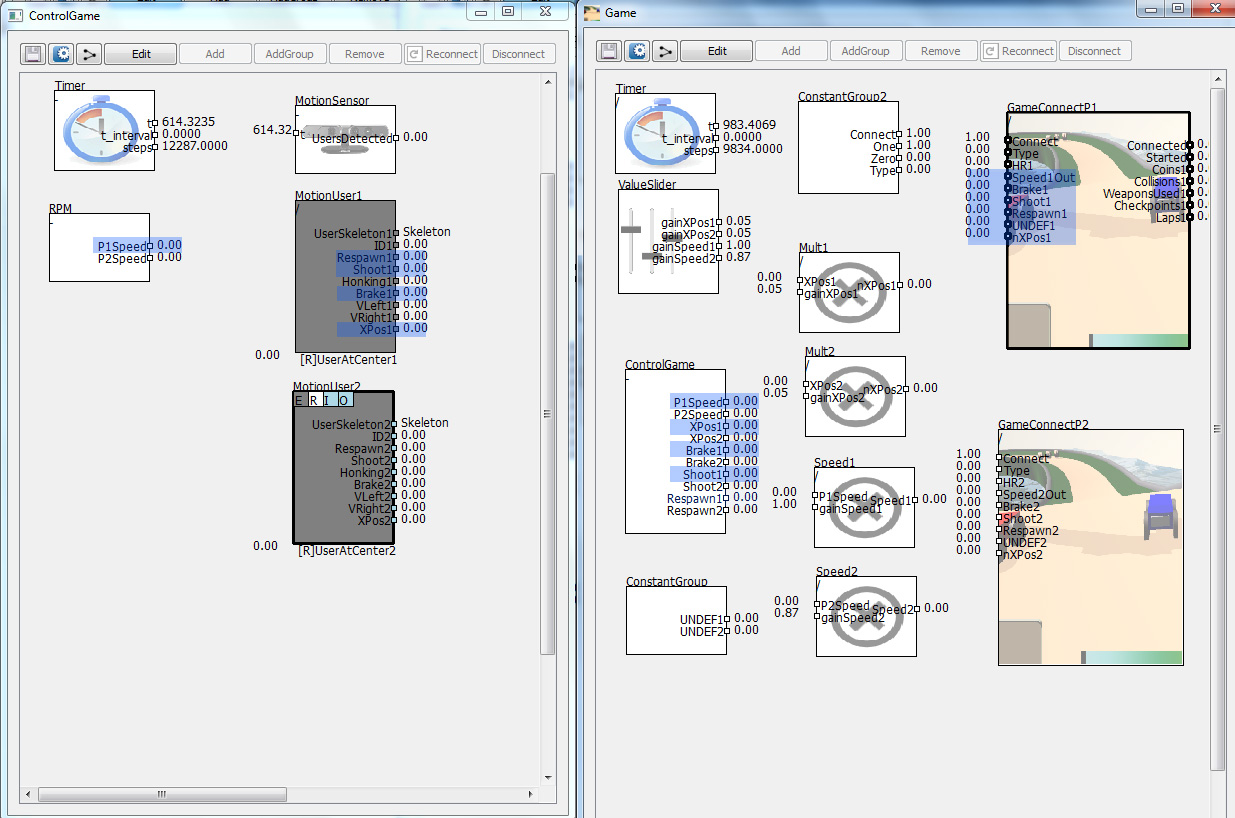
\includegraphics[width=0.4\textwidth]{MDC_motiongamesetup}
 \caption{MDC interface for a setup containing two Unity3D game clients and one motion sensor capturing two players.}
\end{figure}


\section{Biofeedback Adaptations}

The major goal of the game was to promote physical activity, in order to support the personal rehabilitation process. The game mechanics have to work driven by the tracked movement and vital parameters of the player. Our main focus was tracking the heart rate and cycling speed of the participants to recognize physical exhaustion. Playing the game should cause a moderate rise of the player heart rate over time to aerobic training levels. The intensity shouldn't be too low, to obtain a relevant training effect and on the other hand not too high to be dangerous for health. Critical parameters, like the target heart rate ($HR_T$) a player should reach to have an effective training could be assigned individually by a medical skilled supervisor via the initial session options feature of the AutoMedic Framework.
Otherwise, according to \citet{Buttussi2007} the suggested heart rate for aerobic exercise could be automatically set to 60\% - 75\% of his maximum heart rate, calculated with the simple formula $220-age$.
Depending on the current heart rate, several adaptations are made to the game during runtime to either reduce or promote the players physical effort by switching exercise modes. 
\begin{figure}[H]
  \centering
    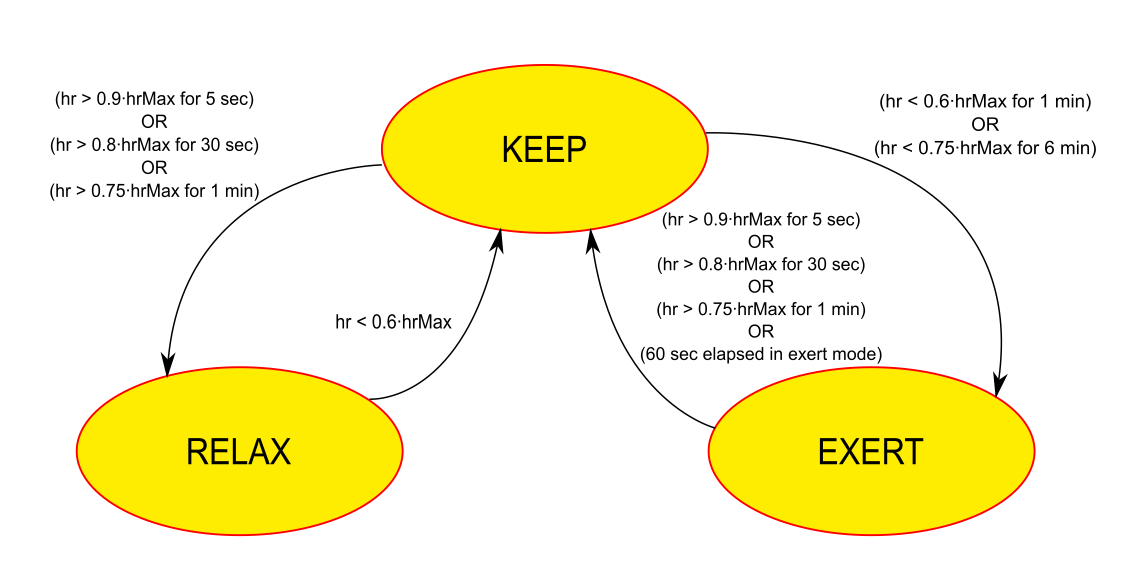
\includegraphics[width=0.4\textwidth]{exerciseautomata}
 \caption{finite state automata to switch among exercise modes as proposed in \cite{Buttussi2007}}
\end{figure}
The different exercise modes influence the supportive power of collected power-ups as well as the Ergometers drag, so that the game can cope with the players' differing stamina levels. Therefore more athletic players have to put more effort in cycling to reach their $HR_T$ just as fast as others. As the participants heart rate gets closer to his individual optimum his game avatar gets faster. Thus the better the training effect, the better the chances for winning the racing game. 
To give the player feedback about his current exertion, the Heads-Up Display (HUD) contained a heart shaped HR indicator which slowly fills up as the players heart rate rises. Upon exceeding the upper limit of the optimum HR, it shows a warning sign. Additionally, screen filling commands were provided telling the user to lower or rise physical effort.




\section{Conclusion and Following Work}
Our goal was to develop a playable multiplayer game prototype with Unity3D embedded in the biofeedback system at the DHZ. The study with the working prototype has shown that playing over a longer period of time does imply a rise in the heart rate of the participation and may therefore work as an alternative to classical rehabilitation approaches. The exergame successfully helped to take the focus away from the serious and exhausting rehabilitation exercise into a lighter game context. Although the data for motion sensor controls was inconclusive, the data collected during sessions played with a gamepad has shown, that participants were able to reach and hold their $HR_T$ with the help of the biofeedback system.
\begin{figure}[H]
  \centering
    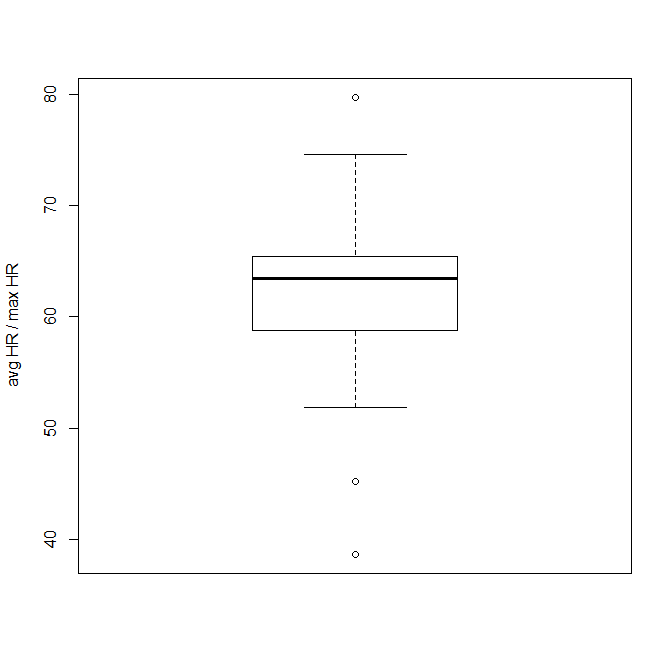
\includegraphics[width=0.4\textwidth]{THRboxplot}
 \caption{Percentage of maximum heartrate reached at average when controlling the game with ergometer and gamepad}
\end{figure}
The game therefore, tries to automatically adapt to the individually fitness and skill level of the players. Weaker players get support over stronger boosts, easier speed gain and simpler steer controls to provide a interesting and challenging game for all players. A medical skilled person could act as instructor and observe the game and players by the server interface or connected MDC application. The recorded biofeedback data gets stored in a database (Couch DB) and could be used for analysing the individual fitness and health status of a player.

Further work is needed to use this game for rehabilitation with children who had heart surgery. Controlling the game with an ergometer may be difficult for children with reduced physical mobility and needs further testing with the according target audience. A possibility to reduce the difficultly of the kart controlling for people with no video game experience, could be to implement a new game mode, where the player could only drive along the track on 3 fixed lines. The player could control his speed by cycling and would automatically drive along the defined track lines. Leaning to the side would cause the kart to jump one line left or right. This gamemode could be played by everyone. The level of challenge in this game mode could be controlled by the number of obstacles, spawned along the 3 track lines. A further advantage of this mode would be, that the game won't be permanently interrupted, because players can't drive against walls or get stuck anywhere.

Besides this, following work could be, to provide all further stored trainings sessions of the player to the game. The server application would be able to visualize the progress of a player over time and is open for more social and customizable features. Through that, the player can see the result of his effort he put in his exercise program. Furthermore, the server application could use the recorded player data to improve and individualize the biofeedback algorithms of the game logic for every player.

The AI could be improved with a state machine and self determining sensor system, which no
longer needs a static path mesh. An obstacle avoiding system, that could automatically detectand calculate an alternative path will also be needed for more complex tracks.
The complete system should be simplified and made playable at home with every common
ergometer. The client, server and MDC applications should be wrapped or merged in one user friendly program, including a simple GUI. This could also help people to do their rehabilitation exercises at home if they are less mobile, but still want to exercise alone in a controlled way. The biofeedback system of the game can help to get better self knowledge about the own fitness status and help to improve self observation during exercising using the sensor system.

\end{multicols}



% The bibliography is printed with \bibliography{}. With the command \bibliographystyle{} a style is picked.

\bibliographystyle{plainnat}
\bibliography{refs/refs}

% To close your document, add the \end{document} command. Everything after this command will not be processed.
\end{document}